\section{Algoritmo Exacto}
\subsection{Implementación del Algoritmo}

\par{Para realizar el algoritmo exacto, utilizamos la técnica de programación de
backtracking. Para ver cuál es el clique con una frontera de mayor
cardinalidad, calculamos la frontera de cada clique que hay en el grafo.
Partimos de una solución en la que el conjunto de nodos es vacío\footnote{
Es debatible si esta solución es válida o no, pero al tener frontera igual
a cero, cualquier solución válida con al menos uno de frontera será mejor.
En todo caso, si el grafo no tiene aristas, se devolverá esta solución vacía.}.
Luego utlizamos recursión para agregar cada posible nodo al conjunto. La
función recursiva se llama a sí misma dos veces: una agregando el i-ésimo
nodo a la solución actual y otra sin agregarlo.}\\

\par{A la función recursiva se le pasan como parámetros la solución actual y
la solución óptima hallada hasta el momento (ambas inicializadas con la
solución vacía). Cada vez que se entra a la función recursiva se evalúa el
tamaño de la frontera de la solución actual y si es mayor a la frontera de
la solución óptima, la solución actual reemplaza a la óptima. Una vez
finalizado el algoritmo se retorna la solución almacenada como óptima. La
solución vacía almacenada como óptima será reemplazada en cuanto se evalúe
cualquier solución con tamaño de frontera mayor a cero. Como cada nodo es una
clique, si el algoritmo retorna la solución vacía significa que el grafo no
tiene aristas.}\\

\par{Con el objetivo de reducir la complejidad del algoritmo exacto se ha
implementado una importante poda. Cuando la función va a llamarse
recursivamente, primero se evalúa si tiene sentido agregar el nodo a la
solución actual, es decir si con el nodo que se agrega, la solución actual
sigue representando una clique. Si con ese nodo no se
forma un clique, luego ese subconjunto de nodos sumado a otros nodos, tampoco
va a ser clique. Por esta razón, se poda toda solución que agregue el nodo
a la solución actual, es decir todo subconjunto de nodos, que no forman una
clique. A continuación se muestra un pseudocódigo del algoritmo exacto basado
en backtracking recursivo.}\\

\begin{algorithm}[H]
	\caption{Pseudocódigo del algoritmo exacto}
	\KwData{\textbf{Grafo} $G(V,E)$}
	\textbf{Solucion} $solucion\_optima$ $\leftarrow$ $solucion\_vacia$\\
	\textbf{Solucion} $solucion\_actual$ $\leftarrow$ $solucion\_vacia$\\
	Recursion(0, $solucion\_optima$, $solucion\_actual$)\\
	\textbf{return} $solucion\_optima$
\end{algorithm}

\begin{algorithm}[H]
	\caption{Llamada recursiva}
	\KwData{\textbf{int} $i$, \textbf{Solucion} $solucion\_optima$, \textbf{Solucion} $solucion\_actual$}
	$solucion\_optima$ $\leftarrow$ Max($solucion\_optima$, $solucion\_actual$)\\
	\If{$i$ = $cantNodos$}{
		Terminar recursion
	}

	\eIf{se\_conecta\_con\_clique($i$, $solucion\_actual$)}{
		Agregar $i$ a $solucion\_actual$\\
		Recursion($i+1$, $solucion\_optima$, $solucion\_actual$)\\
		Quitar $i$ de $solucion\_actual$\\
		Recursion($i+1$, $solucion\_optima$, $solucion\_actual$)
	}{
		Recursion($i+1$, $solucion\_optima$, $solucion\_actual$)
	}
\end{algorithm}

\par{La función $Max$ compara dos soluciones y retorna la de mayor frontera.
$cantNodos$ es la cantidad de nodos del grafo. Cuando el índice del nodo que se
va a agregar $i$ es igual a dicha cantidad, significa que ya no hay más nodos
para agregar y la recursión debe terminar. En otras palabras, se llegó a una
hoja del árbol de backtracking. La función $se\_conecta\_con\_clique$ toma un
nodo $i$ y una solución $S$ y retorna si la solución $S$ seguiría representando
una clique tras agregarle el nodo $i$. Para ello evalúa si existe una arista
entre el nodo $i$ y cada nodo de la clique representada por $S$.}

\subsection{Orden de complejidad}

\par{No puede hacerse mucho análisis respecto al orden de complejidad. El
algoritmo exacto recorre todas las posibles soluciones. Si bien hemos
implementado una poda, en el peor caso (un grafo completo $K_n$) todas las
soluciones serán válidas y todas ellas deberán ser evaluadas. Dado que en
una solución cada nodo puede estar o no estar, la cantidad de soluciones
posibles (la cantidad de subconjuntos del conjunto de nodos) es $2^n$ con
$n$ la cantidad de nodos. Las operaciones realizadas para cada solución son
polinomiales y, por lo tanto no aportan a la complejidad exponencial. La
función $se\_conecta\_con\_clique$ compara $k$ elementos con $k$ la cantidad
de nodos del conunto, que es a lo sumo $n$. Cuando se agregan o se quitan
nodos de una solución, la frontera de dicha solución debe recalcularse. La
complejidad de agragar o quitar un nodo $i$ es $d_G(i)$ (el grado de dicho
nodo, que también puede acotarse superiormente por $n$), ya que deben
evaluarse todas sus aristas. En definitiva, la complejidad del algoritmo
exacto es $2^n * ( n + n + n ) \in$ O($2^n$)}

\subsection{Experimentación}

\subsubsection{Performance}

\par{El archivo $test\_exacto.cpp$ en la carpeta $codigo/exacto$ contiene la
implementación del código que mide los tiempos de ejecución del algoritmo
exacto. Se ejecutó este programa con $N$ = 50,\\$s$ = 1 y $k$ = 10. Es decir,
para cada $n$ entero entre 1 y 50, se generaron 10 grafos aleatorios (
con la función $generar\_aristas\_aleatorias$). Para cada instancia generada se
corrieron dos verisones del algoritmo exacto. Uno con la poda y otro sin ella.
En el siguiente gráfico se muestran los resultados obtenidos.}

\begin{center}
\textbf{Gráfico de performance del algoritmo exacto en\\función de la cantidad
de nodos del grafo}
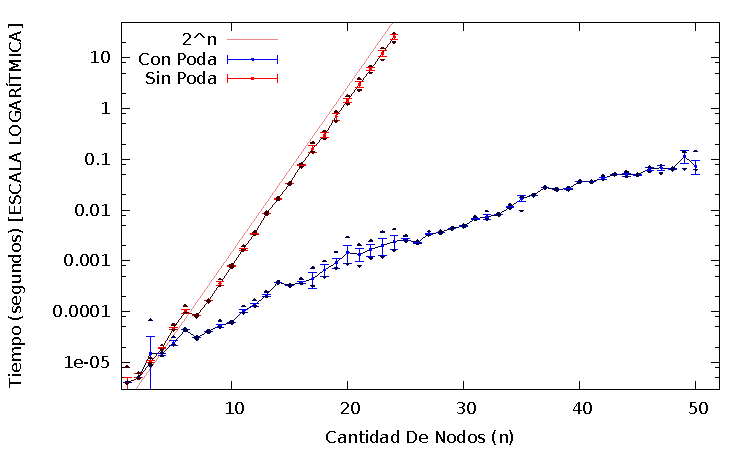
\includegraphics[scale=1.3]{imgs/exacto_50_1_10.pdf}
\end{center}

\par{Cada punto $\bullet$ en el gráfico representa el promedio de los tiempos
medidos para cada una de las 10 ejecuciones de una determinada cantidad de nodos
del grafo. El tamaño del segmento vertical sobre cada punto $\bullet$ representa
su varianza asociada. Además, para cada cantidad de nodos $n$ se graficaron la
máxima medición con $\blacktriangle$ y la mínima medición con
$\blacktriangledown$.}\\

\par{La función graficada con una curva sin puntos es una función exponencial de
base 2. Al estar utilizando escala logarítmica en el eje de ordenadas, esta curva
se ve como una recta. Como se puede observar, la curva definida por la versión
sin poda del algoritmo (la curva resultante de unir los puntos $\bullet$) se
asemeja mucho a tal curva. Mientras que la versión con poda tiene
menores tiempos promedio de ejecución, si bien tiene la misma complejidad.}\\

\par{En la mayotía de los casos, la varianza de ambas versiones es tan pequeña
que apenas puede verse en el gráfico. Esto nos dice que ambas versiones del
algoritmo son estables. Era de esperarse de la versión sin poda, ya que dado
cualquier grafo, la cantidad de soluciones que deben recorrerse es siempre
la misma. Sin embargo, de la versión con poda se esperaba una varianza bastante
superior debido a que la cantidad de soluciones que este debe recorrer depende
en gran medida del grafo entrada.}
